\documentclass{article}
\usepackage{graphicx}
\usepackage{pdfpages}
\usepackage[moderate]{savetrees}
\begin{document}
% Research into:
% - Eigenfaces
% - Sparse Low Rank Bilinear Discriminative Model
% - What are liveness tests
% - How can we test a system that we create?
% - What test data is available? ROSE-Youtu Face liveness detection dataset
% - Deep Learning based face liveness detection in videos
% - Cameras used: mobile cameras (most methods use average resolution images from webcams or camera phone)
% - "Deep learning based face liveness detection in videos" https://ieeexplore.ieee.org/document/8090202/
% - Ideas: texture based - an image of a face will have the facial textures, while the texture of a piece of paper is very different.
% - Video vs Photo. Wtih a video, you don't just use the subject image, but also factor in movement and changes.
    
    \paragraph{Title}
        Facial Authentication System for the Web
    \paragraph{Project Type}
        Computer Vision, Image Processing and Security
    \paragraph{Description}
        - Traditional username and password focused approaches to authentication have drawbacks (such as password leaks)
        - Existing biometric methods have their problems when applied to a web system, due to the transparency of web systems.
        - Overcoming the transparency hurdle would produce a secure method of authentication for the web, using faces of users.
        - Using multiple methods of facial recognition, facial liveness tests, coupled with implementation details, these can be used to create a robust
        authentication service.
    \paragraph{Preliminary Preparation}
        \begin{itemize}
            \item Existing biometric web-based authentication methods, how do they work, what are their benefits/drawbacks?
            \item What spoofing methods could be undertaken, and how can we prevent these?
            \item What are the privacy concerns regarding a facial recognition approach, and how can these be mitigated?
            \item How can this be integrated into a web service?
            \item Use as a single sign on service (SSO). What protocols are there, how do they work, how can we integrate our system into these standards?
        \end{itemize}
    \paragraph{Minimum Objectives}
        \begin{itemize}
            \item Server that recognises a user given their face (therefore carrying out authentication), generating a token for a user given their face. This token can be used for authorization.
            \item Client side that accepts user video, and transmits it to the main application for further processing
            \item Main server that utilises microservices to do the large amounts of processing necessary at scale.
        \end{itemize}
    \paragraph{Intermediate Objectives}
        \begin{itemize}
            \item CNN-based liveness for a photograph of a user's face
            \item Reference image facial matching, using a CNN.
        \end{itemize}
    \paragraph{Advanced Objectives}
        \begin{itemize}
            \item Preventing replay attacks - preventing someone from intercepting someone's facial image using image metadata methods.
            \item Lipreading speech-based liveness check
            \item SAML2 protocol implemented, to provide an SSO to many other applications.
        \end{itemize}
    \paragraph{References}
        \begin{itemize}
            \item Keras (https://keras.io) for Machine Learning
            \item OpenCV (https://opencv.org/) for image Processing
        \end{itemize}

   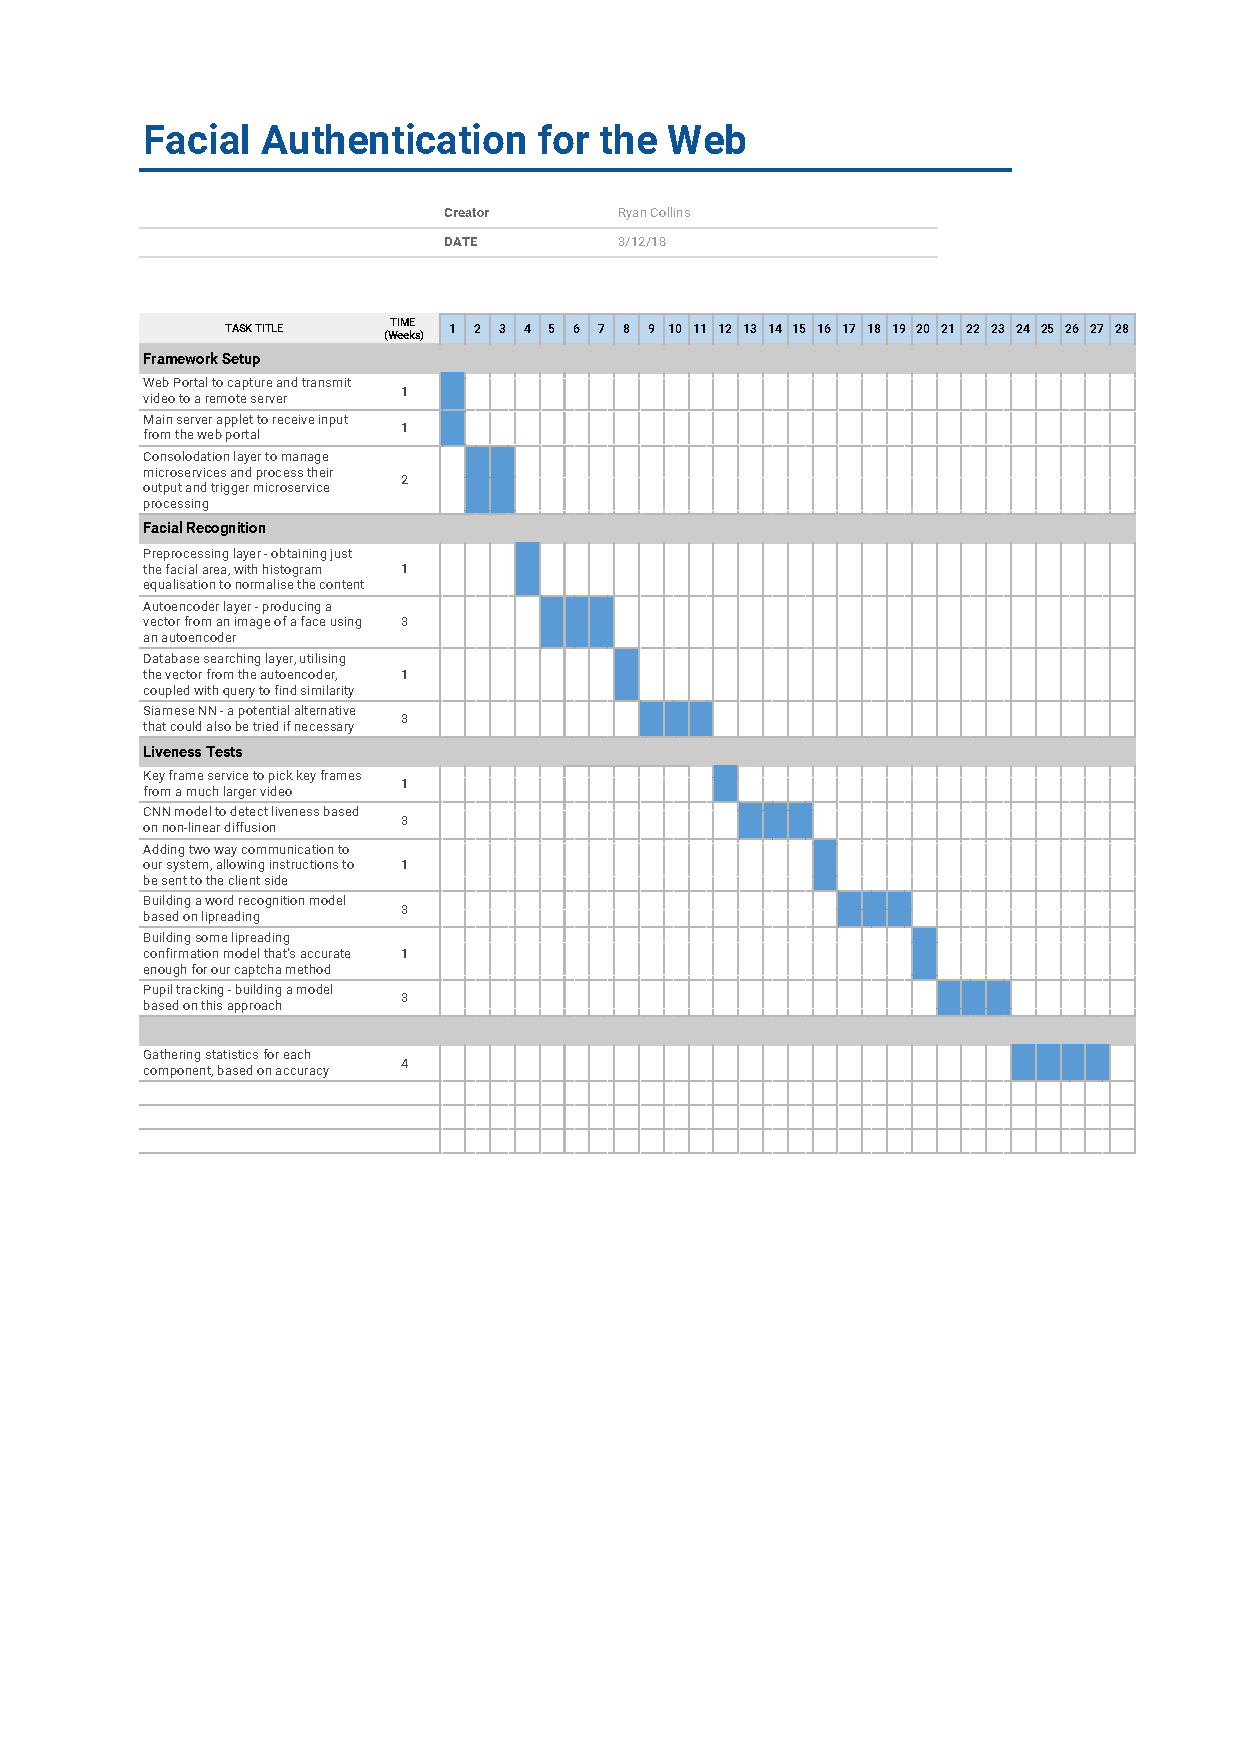
\includepdf{gantt.pdf}
\end{document}